\section{Implementation}
\label{sec:implementation}

This section describes the implementation of CPSForge. The system is built around a real Siemens S7 PLC connected to Factory~I/O (a software-based process emulator), with logic engineered in TIA Portal~v17. All experiments execute in a PLC-in-the-loop setting where the controller runs real scan cycles against emulated plant I/O.

\subsection{Hardware and Process Setup}

The controller layer consists of a Siemens S7-1200 PLC deployed with logic created in TIA Portal~v17. The PLC communicates over Ethernet at a fixed IP address (192.168.0.1). Factory~I/O serves as the process emulator, providing realistic industrial scenes with sensors, actuators, and stateful physical interaction. The PLC interacts with Factory~I/O through the normal control loop, while CPSForge observes and mediates selected control-relevant variables through an external middleware bridge implemented using the python-snap7 library~\cite{snap7}.

The current evaluation covers three Factory~I/O scenes:

\begin{itemize}[leftmargin=1.5em]
    \item \textbf{Level Control (Scene~12):} a continuous tank filling and draining process with 15 tags (fill valve, discharge valve, liquid level, setpoints, enable), controlled by a PID loop. Attack surfaces: setpoint shift and actuator override.
    \item \textbf{Sorting by Height (Scene~19):} a discrete 2-way sorting conveyor with 30 tags (entry conveyor, transfer left/right, load/unload actuators, height sensors, enable). Attack surfaces: wrong transfer gate activation, conveyor stall.
    \item \textbf{Sorting by Weight (Scene~20):} a discrete 3-way weight-threshold sorting process with 35 tags (conveyors, weight sensor, threshold setpoints, diverters). Attack surfaces: threshold shift (missort), wrong diverter (jam), conveyor stall.
\end{itemize}

Figure~\ref{fig:scenes} shows two representative scenes as rendered in Factory~I/O. Level Control (Scene~12) is a closed-loop continuous process: a single tank is filled and drained by proportional valves whose positions are computed by a PID controller tracking a configurable liquid-level setpoint. Sorting by Weight (Scene~20) is a discrete classification process: items travel along an entry conveyor, are weighed on a scale, and are diverted left, right, or forward by pneumatic pushers based on configurable weight thresholds.

\begin{figure*}[t]
    \centering
    \begin{subfigure}[t]{0.48\textwidth}
        \centering
        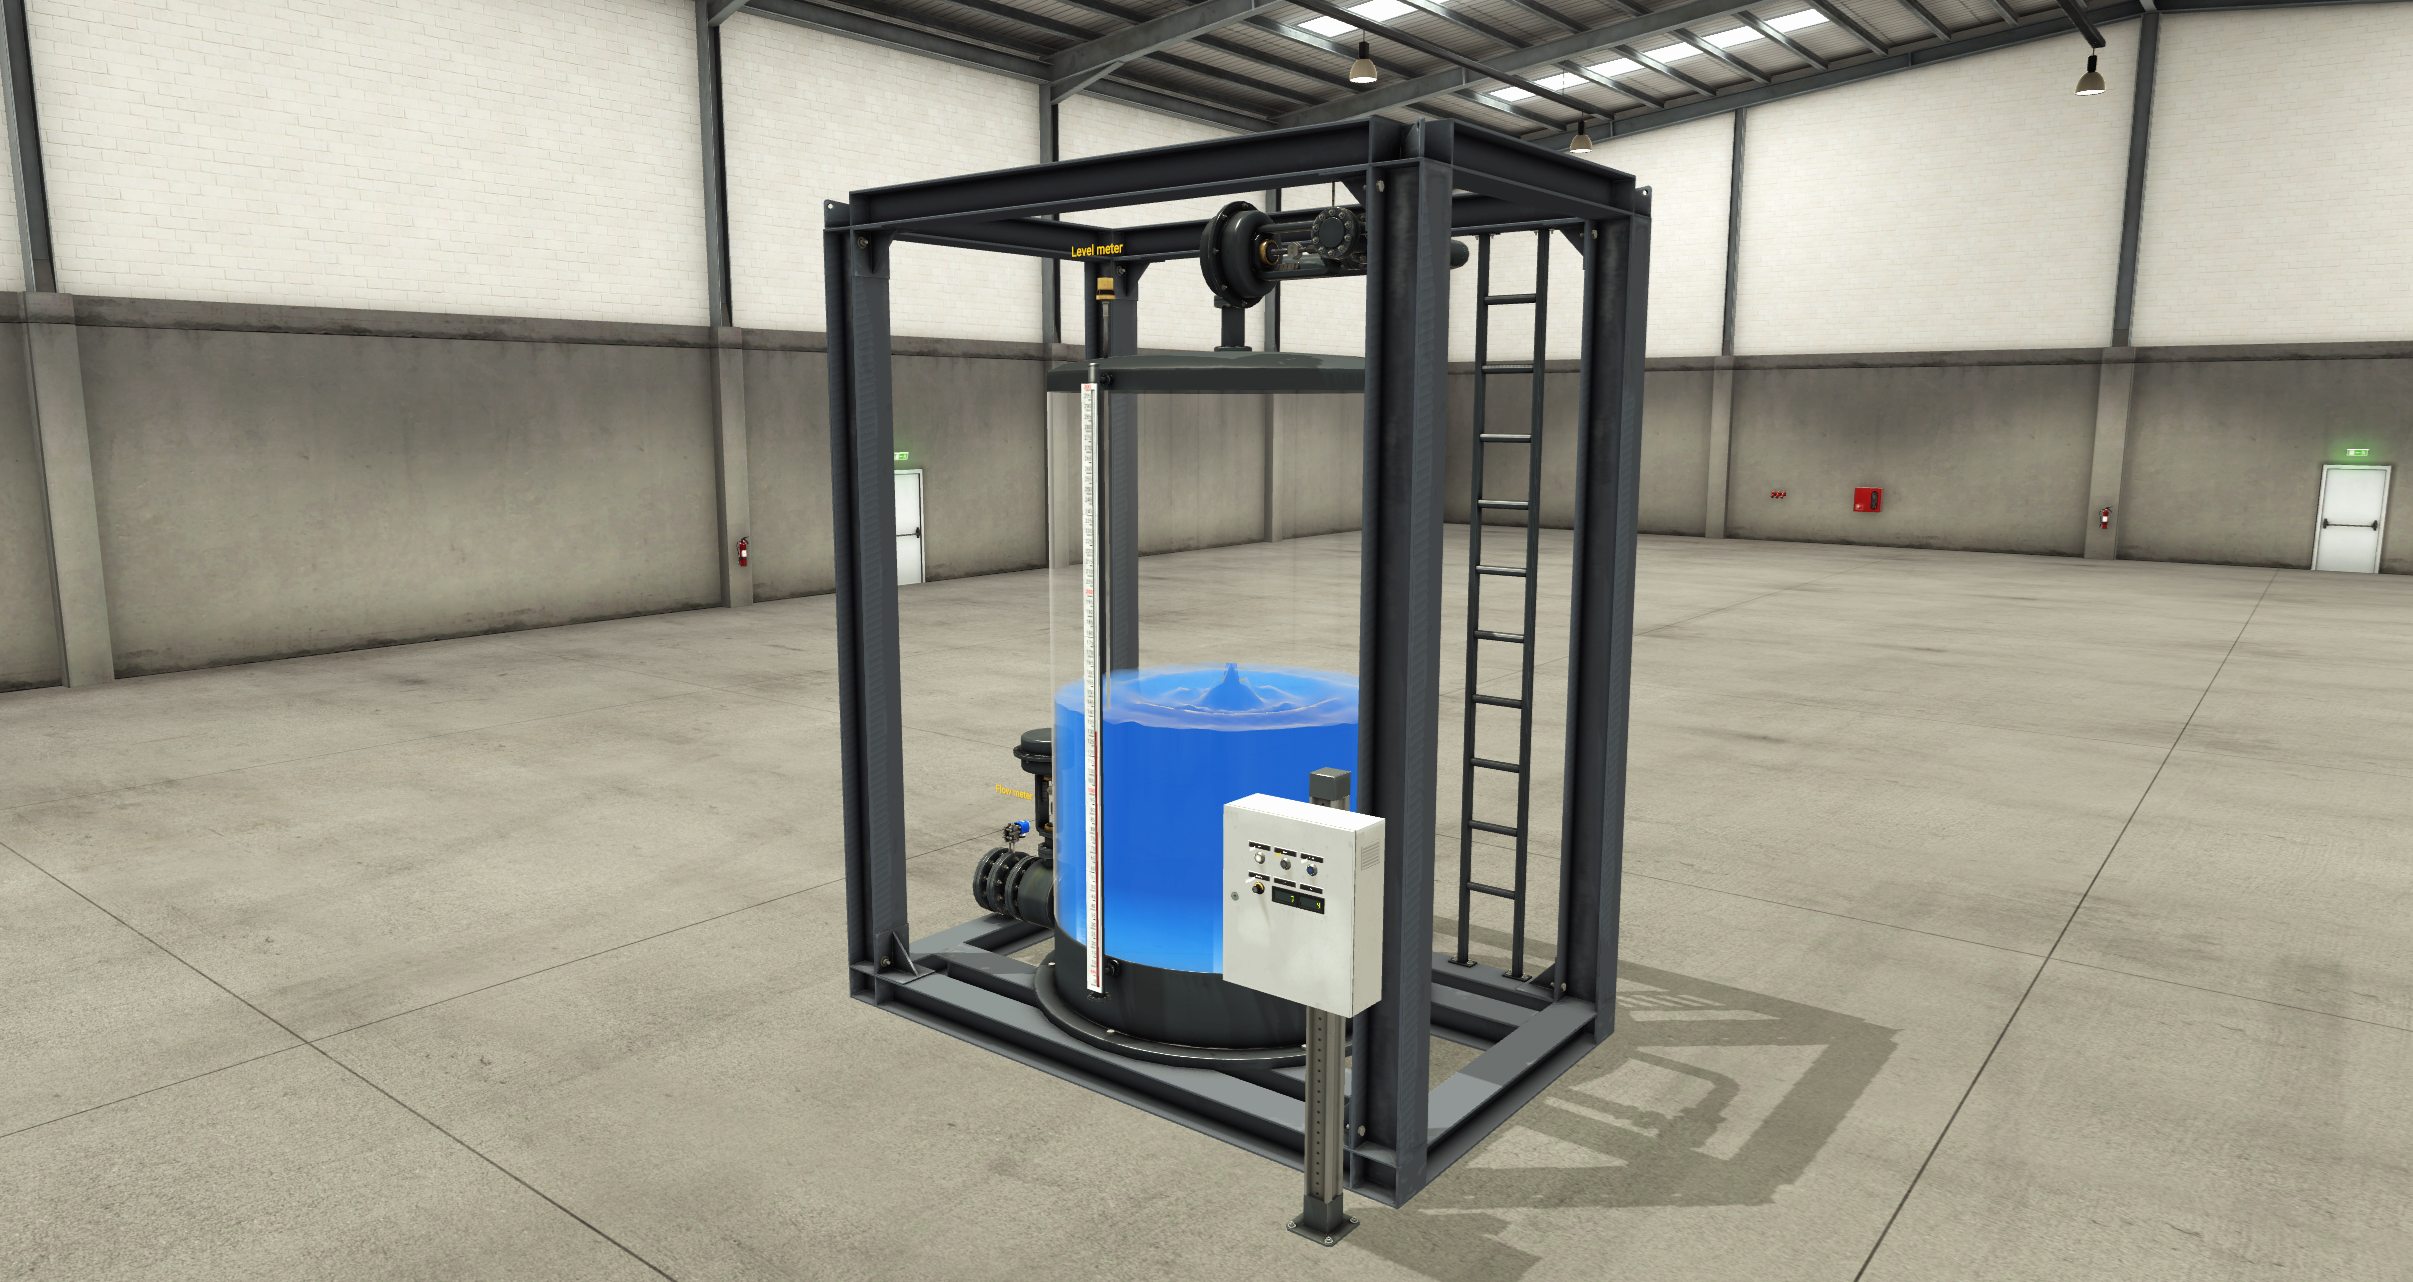
\includegraphics[width=\linewidth]{images/s12.png}
        \caption{\textbf{Level Control (Scene~12).} A continuous tank process controlled by a PID loop. The attacker can shift the liquid-level setpoint, override fill or drain valves, or disable the controller to cause overflow or drain events.}
        \label{fig:scene-s12}
    \end{subfigure}
    \hfill
    \begin{subfigure}[t]{0.48\textwidth}
        \centering
        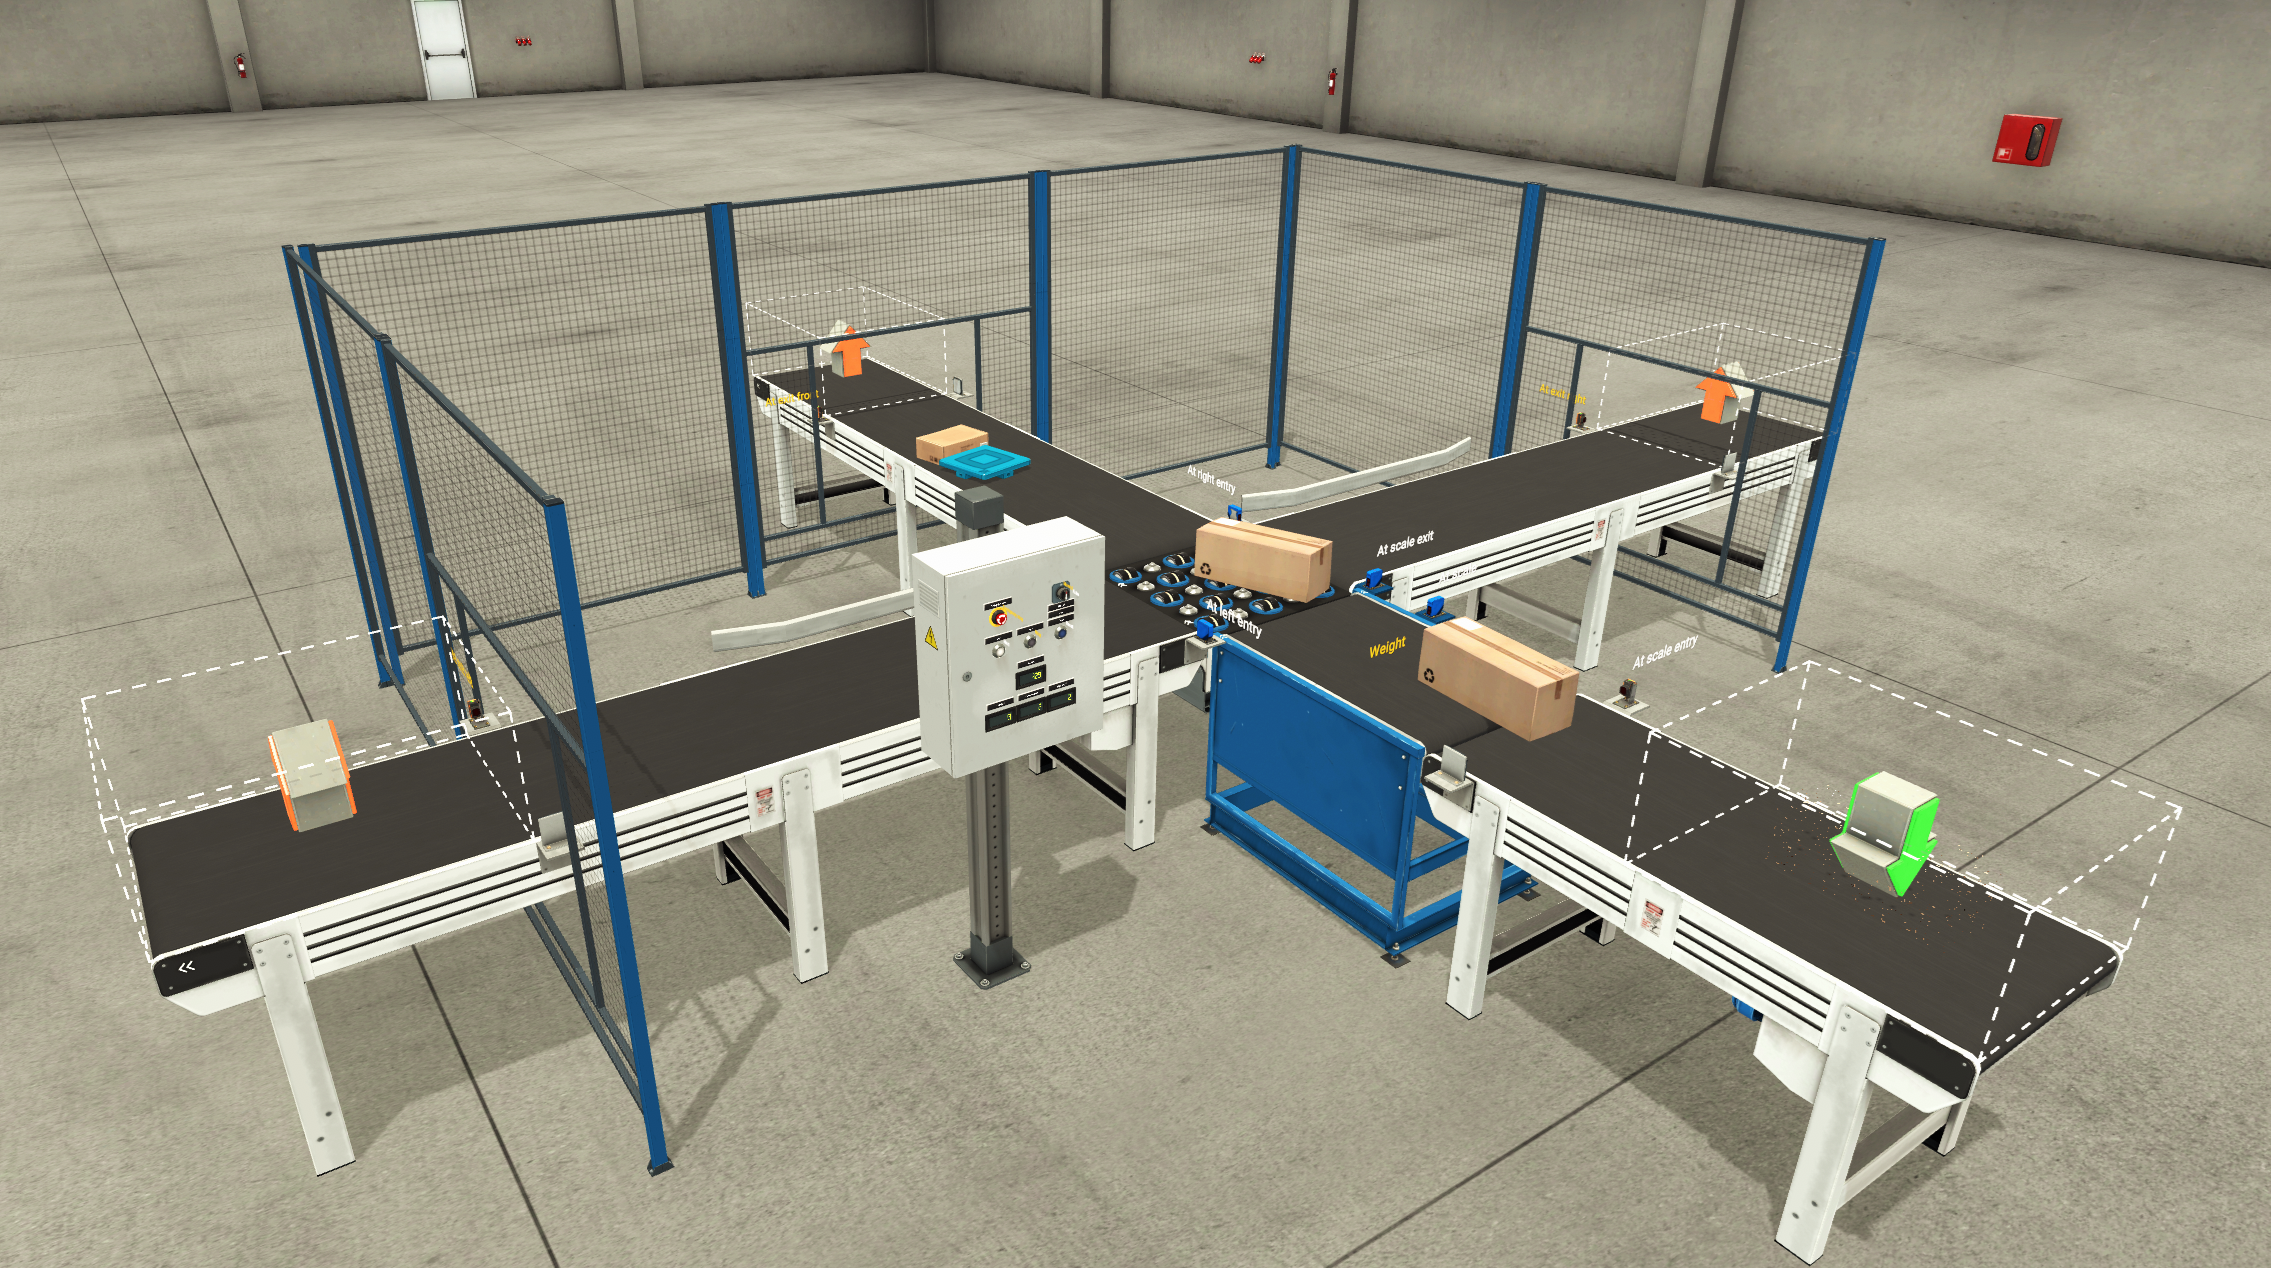
\includegraphics[width=\linewidth]{images/s20.png}
        \caption{\textbf{Sorting by Weight (Scene~20).} A threshold-based discrete sorting process. The attacker can manipulate weight classification thresholds or diverter actuators to mis-sort items and disrupt throughput.}
        \label{fig:scene-s20}
    \end{subfigure}
    \caption{Two representative Factory~I/O industrial scenes used in CPSForge experiments. Both scenes are driven by a real Siemens S7-1200 PLC (192.168.0.1) with control logic deployed via TIA Portal~v17. Level Control provides a continuous-process attack surface with setpoint and actuator targets; Sorting by Weight provides a discrete-classification attack surface with classifier threshold and diverter targets.}
    \label{fig:scenes}
\end{figure*}

\subsection{Middleware Bridge}

A Python-based middleware layer communicates with the PLC via python-snap7, providing cyclic telemetry collection, action compilation, and structured logging. The middleware reads relevant tags at a configurable polling interval (default 500\,ms), constructs structured plant snapshots using Pydantic data models, and forwards context to the attacker and defender modules. Approved attack actions are translated into bounded PLC writes through the safety shield.

Each polling interval records: timestamp, scene identifier, sensor values, actuator states, controller mode bits, alarm status, setpoints, active attack context, shield decisions, and detector outputs. These records form the basis for both online monitoring and offline replay.

\subsection{Scene Profiles}

Each Factory~I/O scene is represented as a configurable YAML profile that defines tag metadata, process descriptions, writable variables exposed to the attacker, allowed attack types, safety invariants, reset behavior, and sampling interval. This scene abstraction allows the core framework to remain independent of any one process while capturing scene-specific semantics.

\subsection{Attack Representation}
\label{sec:impl:attack}

CPSForge does not permit attack modules to manipulate raw memory areas directly. Instead, every attacker outputs a structured \texttt{AttackAction} object containing the fields listed in Table~\ref{tab:action-fields}. This representation constrains the action space to meaningful process operations, enables validation by the shield, and makes experiments easier to replay and analyze.

\begin{table}[t]
\centering
\caption{Fields of a structured \texttt{AttackAction} object. Every attack---scripted, random, or LLM-generated---must populate these fields before submission to the safety shield.}
\label{tab:action-fields}
\small
\begin{tabular}{lp{5.2cm}}
\toprule
\textbf{Field} & \textbf{Description} \\
\midrule
\texttt{attack\_type} & One of: \texttt{actuator\_override}, \texttt{setpoint\_shift}, \texttt{sensor\_spoof}, \texttt{sequence\_perturbation}, \texttt{timing\_delay} \\
\texttt{target} & Symbolic tag name (e.g., \texttt{fill\_valve}, \texttt{setpoint\_in}); raw PLC addresses are never exposed \\
\texttt{mode} & Write semantics: \texttt{override} (direct), \texttt{offset} (additive), \texttt{freeze} (hold current), \texttt{zero} (force 0/False) \\
\texttt{value} & Numeric or boolean value to write \\
\texttt{duration\_ms} & How long the override persists (1--15\,s typical) \\
\texttt{rationale} & Attacker's stated intent (used for logging and LLM prompt history) \\
\texttt{expected\_effect} & Predicted physical consequence \\
\texttt{confidence} & Attacker's self-assessed probability of success [0,\,1] \\
\texttt{source} & Origin: \texttt{random}, \texttt{llm\_static}, or \texttt{llm\_online} \\
\bottomrule
\end{tabular}
\end{table}

The \textbf{Action Compiler} translates each approved action into a concrete PLC write dictionary \texttt{\{tag\_name: value\}}. In \texttt{override} mode the value is written directly; in \texttt{offset} mode it is added to the current sensor reading; \texttt{freeze} re-writes the tag's current value each cycle; and \texttt{zero} forces the tag to 0 or False. The compiler never bypasses the safety shield---only shield-approved actions reach it.

\paragraph{Scripted attack scripts.}
The scripted attacker loads a deterministic sequence from a per-scene YAML configuration file (or built-in defaults). Each script entry is a complete \texttt{AttackAction} template. For example, the Level Control scripted attack executes four actions in sequence:
\begin{enumerate}[leftmargin=1.5em, nosep]
  \item \textbf{Setpoint shift} on \texttt{setpoint\_in}~$\to$~9.5 for 12\,s --- drives the fill valve toward its maximum, risking tank overflow.
  \item \textbf{Actuator override} on \texttt{fill\_valve}~$\to$~10.0 for 8\,s --- forces the fill valve fully open, flooding the tank regardless of the controller setpoint.
  \item \textbf{Actuator override} on \texttt{discharge\_valve}~$\to$~10.0 for 10\,s --- forces the drain fully open, rapidly emptying the tank.
  \item \textbf{Actuator override} on \texttt{enable}~$\to$~False for 15\,s --- disables the PLC control loop entirely, freezing all valve outputs.
\end{enumerate}
Similar scripts are defined for each scene. For Sorting by Weight, the script shifts the \texttt{light\_thresh} and \texttt{heavy\_thresh} setpoints to mis-sort items, then overrides the \texttt{send\_left} diverter to force all items left regardless of weight. For Filling Tank, the script overrides \texttt{fill\_valve}~$\to$~False to stall the fill cycle, then forces \texttt{drain\_valve}~$\to$~True during the fill phase to violate the mutual-exclusion invariant. Each script is designed to exercise distinct attack surfaces and to trigger different combinations of safety rules and detector alerts.

\paragraph{Random attacker.}
The random attacker selects a target tag uniformly from the scene's declared attack surface, chooses an attack type from a configured whitelist, draws a value uniformly within the tag's \texttt{[min\_value, max\_value]} bounds, and selects a duration in $[1\,\text{s},\,15\,\text{s}]$. The PRNG seed is recorded per run for full reproducibility.

\paragraph{LLM attacker.}
The LLM attacker receives a structured prompt containing: the scene profile (tag names, types, ranges, and descriptions), the current plant snapshot (all sensor and actuator readings), the attacker objective (e.g., ``cause the tank level to deviate beyond normal bounds while remaining undetected''), and the list of allowed attack types. The LLM must return its response as a valid JSON object matching the \texttt{AttackAction} schema. A normalization layer maps common aliases (e.g., \texttt{actuator\_takeover}~$\to$~\texttt{actuator\_override}), repairs malformed numeric fields, and unwraps nested JSON objects. Invalid responses trigger automatic retries with schema-correction prompts (up to 3 retries). Crucially, the LLM never receives raw PLC addresses or memory offsets---only symbolic tag names.

\subsection{LLM Defender}

The LLM defender uses the same model architecture and context pipeline as the attacker but with a defense-oriented prompt. For each proposed PLC write that passes the safety shield, the defender LLM receives: the current process state, the proposed write (target tag, value, duration, action type), scene description, control objective, and inferred process phase. It outputs a JSON decision: \texttt{decision} (allow/block), \texttt{suspicion\_score} (0--1), and \texttt{reasoning}. Writes with suspicion score $\geq 0.5$ or explicit ``block'' decisions are rejected. On parse failure, the defender defaults to ``allow'' to avoid blocking legitimate controller writes. This creates a symmetric LLM-vs-LLM evaluation where the same model serves as both attacker and defender.

\subsection{Safety Shield Implementation}
\label{sec:impl:shield-impl}

The shield evaluates seven sequential checks before a candidate action executes: (1)~whitelist check (target tag must be in the attack surface), (2)~range check (value within bounds), (3)~duration cap, (4)~cooldown window, (5)~invariant check (hard safety rules), (6)~interlock check (blocks writes when condition tags indicate unsafe state), and (7)~mode gate. The shield emits a structured \texttt{ShieldDecision} with approval status, violated rules, and a rollback plan (original tag values for automatic restoration after attack expiry).

The defense chain applies sequentially after the shield: PhaseAwareShield $\to$ IntentConsistencyChecker $\to$ LLM Defender $\to$ Execute. Each stage can independently block a write. Figure~\ref{fig:shield-flow} shows the decision flow.

\begin{figure}[t]
    \centering
    \begin{tikzpicture}[
        >=Stealth,
        node distance=0.3cm,
        every node/.style={font=\scriptsize},
        stepbox/.style={draw, rounded corners=2pt, minimum width=2.4cm, minimum height=0.45cm, align=center, thick},
        dec/.style={draw, diamond, aspect=2.5, inner sep=1pt, align=center, thick, font=\scriptsize},
        arr/.style={->, thick, >=Stealth},
    ]
    \node[stepbox, fill=red!10] (input) {Proposed Action};
    \node[dec, fill=yellow!15, below=0.4cm of input] (wl) {Target on\\whitelist?};
    \node[dec, fill=yellow!15, below=0.5cm of wl] (range) {Value in\\range?};
    \node[dec, fill=yellow!15, below=0.5cm of range] (dur) {Duration\\$\leq$ cap?};
    \node[dec, fill=yellow!15, below=0.5cm of dur] (interlock) {Interlocks\\OK?};
    \node[stepbox, fill=green!15, below=0.4cm of interlock] (approve) {\textbf{Approved}\\+ rollback plan};
    \node[stepbox, fill=red!15, right=1.2cm of range] (reject) {\textbf{Rejected}\\+ reason log};

    \draw[arr] (input) -- (wl);
    \draw[arr] (wl) -- node[left, font=\tiny]{\checkmark} (range);
    \draw[arr] (wl.east) -- ++(0.3,0) |- node[above, near start, font=\tiny]{$\times$} (reject);
    \draw[arr] (range) -- node[left, font=\tiny]{\checkmark} (dur);
    \draw[arr] (range.east) -- node[above, font=\tiny]{$\times$} (reject);
    \draw[arr] (dur) -- node[left, font=\tiny]{\checkmark} (interlock);
    \draw[arr] (dur.east) -- ++(0.3,0) |- node[above, near start, font=\tiny]{$\times$} (reject);
    \draw[arr] (interlock) -- node[left, font=\tiny]{\checkmark} (approve);
    \draw[arr] (interlock.east) -- ++(0.3,0) |- node[below, near start, font=\tiny]{$\times$} (reject);

    \end{tikzpicture}
    \caption{Safety shield decision flow. Each proposed action must pass four sequential checks before approval. Any failure produces a structured rejection with explicit reasons.}
    \label{fig:shield-flow}
\end{figure}

\subsection{Defender Stack}
\label{sec:impl:defenders}

The defender stack comprises six detectors spanning rule-based, statistical, and learned categories. All implement a common interface (\texttt{observe}, \texttt{detect}, \texttt{reset}) and emit structured \texttt{DetectionEvent} objects.

\textbf{Rule-based detectors.} The \emph{threshold detector} fires when a tag crosses a configured boundary (e.g., \texttt{level\_meter~$>$~9.0}). The \emph{invariant detector} evaluates boolean process constraints expressed over tag values (e.g., ``fill valve must not exceed 9.0 when level exceeds 9.0''); violations indicate physically inconsistent states.

\textbf{Statistical detectors.} The \emph{CUSUM detector}~\cite{page1954continuous} tracks cumulative sums to detect small persistent mean shifts. The \emph{Isolation Forest}~\cite{liu2008isolation} isolates anomalies via random partitioning with sub-second latency.

\textbf{Learned detectors.} The \emph{One-Class SVM}~\cite{scholkopf2001estimating} scores snapshots against a learned kernel-space boundary. The \emph{LSTM autoencoder}~\cite{malhotra2016lstm} detects temporal anomalies via reconstruction error on sliding windows.

Rule-based detectors require only scene-specific configuration. ML-based detectors are trained offline on 300-step baseline traces ($\approx$2.5~minutes).

\subsection{LLM Integration}
\label{sec:impl:llm}

CPSForge uses in-process HuggingFace \texttt{transformers} inference with 4-bit NF4 quantization. The primary model is Qwen2.5-3B-Instruct (${\sim}$6\,GB VRAM); cross-model comparisons use Qwen3-1.7B and SmolLM3-3B. All models run locally on an NVIDIA RTX~A4000 (16\,GB). The integration layer includes versioned prompt templates, JSON schema validation with automatic repair of malformed outputs, and structured logging for reproducibility.

\subsection{Agent Mode}
\label{sec:impl:agent}

The attacker and defender run as independent processes communicating through typed message queues. A coordinator polls PLC tags, broadcasts snapshots to both agents, validates proposed writes through the safety shield, and executes approved actions. All decisions are logged for post-hoc analysis.

\subsection{Data Management}
\label{sec:impl:artifacts}

Each experiment run produces structured artifacts: a Parquet trace file (one row per poll step with all tags, attack context, and detection events), JSON files for attacks, shield decisions, and detections, plus aggregated metrics. After all runs complete, summary files enable automated metric extraction. All values reported in this paper are computed from these artifacts.

The pipeline is fully operational: 333~evaluation runs have been executed against the real PLC across three Factory~I/O scenes using random, online MITM LLM, static LLM, and frontier API attackers. Results are presented in Section~\ref{sec:evaluation}.